% Figure for scale_lanes_deck: Runtime 1 : N sessions, session 1 : 1 microVM.
% Build: xelatex lanes_fig03_concepts.tex  (-> .pdf, included by ../scale_lanes_deck.md)
\documentclass[tikz,border=4pt]{standalone}
\usepackage{fontspec}
\setmainfont{DejaVu Sans}
\setmonofont{DejaVu Sans Mono}
\usetikzlibrary{positioning,arrows.meta,fit,backgrounds,calc,decorations.pathreplacing}
\definecolor{slime}{RGB}{230,230,230}
\definecolor{host}{RGB}{214,216,240}
\definecolor{gpu}{RGB}{255,236,204}
\definecolor{vm}{RGB}{214,238,220}
\definecolor{ac}{RGB}{255,246,230}
\definecolor{bad}{RGB}{245,205,205}
\definecolor{ink}{RGB}{40,40,90}
\begin{document}
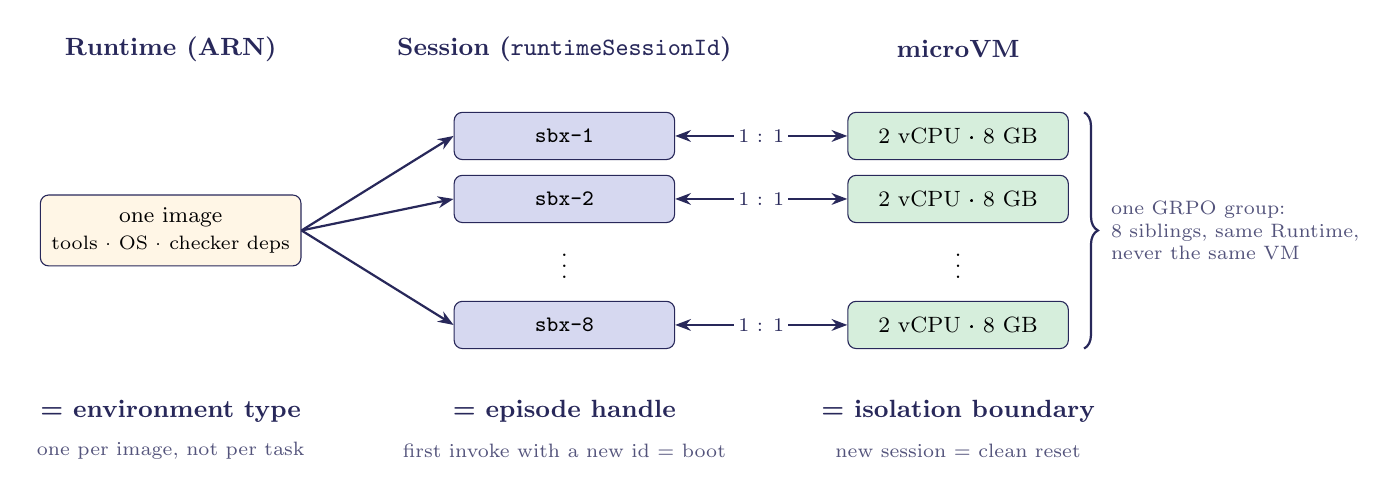
\begin{tikzpicture}[
  font=\footnotesize,
  box/.style={draw=ink, rounded corners=3pt, fill=#1, align=center, inner sep=4pt, minimum height=0.9cm, minimum width=2.8cm},
  line/.style={thick, draw=ink, -{Stealth[length=2mm]}},
  dline/.style={thick, draw=ink, {Stealth[length=2mm]}-{Stealth[length=2mm]}},
  head/.style={font=\small\bfseries, text=ink, align=center},
  lab/.style={font=\scriptsize, text=ink, fill=white, inner sep=1.5pt, align=center},
  note/.style={font=\scriptsize, text=ink!80, align=center},
  region/.style={draw=ink!60, dashed, rounded corners=6pt, inner sep=8pt},
]

\node[head] at (0,1.5) {Runtime (ARN)};
\node[head] at (5,1.5) {Session (\texttt{runtimeSessionId})};
\node[head] at (10,1.5) {microVM};
\node[box=ac] (r) at (0,-0.8) {one image\\\scriptsize tools · OS · checker deps};
\foreach \i/\y/\t in {1/0.4/sbx-1, 2/-0.4/sbx-2, 3/-2.0/sbx-8} {
  \node[box=host, minimum height=0.6cm] (s\i) at (5,\y) {\texttt{\t}};
  \node[box=vm, minimum height=0.6cm]   (v\i) at (10,\y) {2 vCPU · 8 GB};
  \draw[line] (r.east) -- (s\i.west);
  \draw[dline] (s\i) -- node[lab] {1 : 1} (v\i);
}
\node at (5,-1.15) {$\vdots$}; \node at (10,-1.15) {$\vdots$};
\draw[decorate, decoration={brace, amplitude=5pt}, thick, ink] (11.6,0.7) -- (11.6,-2.3)
  node[midway, right=6pt, note, align=left] {one GRPO group:\\8 siblings, same Runtime,\\never the same VM};
\node[note, font=\small\bfseries, text=ink] at (0,-3.1)  {= environment type};
\node[note, font=\small\bfseries, text=ink] at (5,-3.1)  {= episode handle};
\node[note, font=\small\bfseries, text=ink] at (10,-3.1) {= isolation boundary};
\node[note] at (0,-3.6)  {one per image, not per task};
\node[note] at (5,-3.6)  {first invoke with a new id = boot};
\node[note] at (10,-3.6) {new session = clean reset};
\end{tikzpicture}
\end{document}
